% ch-a4-13.tex —— 第 4 篇（Emerton--Gee--Hellmann）续片，底本 PDF 324--335 = 印刷页 311--322

\ysrc{311}……$(\GG_m)_t$ 到 $(\GG_m)^f$ 的嵌入，可得该映射由下式给出
\[
(a_0,\dots,a_{f-1})\mapsto\Bigl(\sum_j a_j,\bigl(\sum_{j\neq i-1}a_j-a_{i-1}\bigr)_{i=0}^{f-1}\Bigr)
=\Bigl(\sum_j a_j,\bigl(\sum_{j=0}^{f-1}a_j-2a_{i-1}\bigr)_{i=0}^{f-1}\Bigr).
\]
于是可见 (7.6.7) 是嵌入，并且可以由 $\Z^{f+1}$ 中的坐标还原各个 $a_i$；显式地，（左）逆由下式给出
\[
(b,b_0,\dots,b_i,\dots,b_{f-1})\mapsto\frac12(b-b_1,\dots,b-b_{i+1},\dots,b-b_0).
\]
现在坐标 $(b,b_0,\dots,b_{f-1})$ 是典范的，至多相差对 $b_i$ 的置换（对应于对 $\sigma_i$ 的重新标号）；因此同构 $\mathrm{Pic}(\XX(\sigma))\cong\Z^f$ 是典范的，至多相差对坐标 $a_i$ 的置换。

\subsubsection*{7.6.8.\quad 驯顺型}
若 $\tau$ 是 $\Q_{p^f}$ 的驯顺惯性型（tame inertial type），则相应的 $K$-表示 $\sigma^{\mathrm{crys}}(\tau)$ 通过 $\mathrm{GL}_2(k_F)=\mathrm{GL}_2(\F_{p^f})$ 分解。若 $\sigma^{\mathrm{crys}}(\tau)^\circ$ 是 $\sigma^{\mathrm{crys}}(\tau)$ 中的 $K$-不变格（lattice），则其约化的 Jordan--Hölder 因子的多重集事实上是一个互异 Serre 权（Serre weight）的集合，它不依赖格的具体选取；我们把它记作 $\mathrm{JH}\bigl(\ol{\sigma^{\mathrm{crys}}(\tau)}\bigr)$。若 $\tau$ 进一步充分 generic，则 $\mathrm{JH}\bigl(\ol{\sigma^{\mathrm{crys}}(\tau)}\bigr)$ 恰由 $2^f$ 个权组成。

我们写 $\XX(\tau)=\bigcup_{\sigma\in\mathrm{JH}(\ol{\sigma^{\mathrm{crys}}(\tau)})}\XX(\sigma)$；这是 $\XX_{\mathrm{red}}$ 的闭子叠（closed substack）。

\begin{thm}{7.6.9}\label{thm:a4-7-6-9}
若 $\tau$ 是充分 generic 的驯顺型，则 $\mathrm{Pic}(\XX(\tau))\cong\Z^{2^f}$。
\end{thm}

事实上，限制映射的乘积
\[
\mathrm{Pic}(\XX(\tau))\hookrightarrow\prod_{\sigma\in\mathrm{JH}(\ol{\sigma^{\mathrm{crys}}(\tau)})}\mathrm{Pic}(\XX(\sigma))
\]
是单射，并且可以把 $\mathrm{Pic}(\XX(\tau))$ 的像等同于目标的一个特定子群。

\subsubsection*{7.6.10.\quad 函子的取值}
[EGS15] 的结果表明：若 $\sigma$ 是 generic 的 Serre 权，或 $\sigma^{\mathrm{crys}}(\tau)^\circ$ 是充分 generic 的驯顺型 $\tau$（其行列式等于 $\zeta|_{\OO_F^\times}$）的适当选取的格，则由适当的 Shimura 曲线背景构造出的拼接模 $M_\infty(\sigma)$ 与 $M_\infty\bigl(\sigma^{\mathrm{crys}}(\tau)^\circ\bigr)$ 在其支撑上秩一自由。Serre 猜想的权部分，与可能 Barsotti--Tate 表示的（几何）Breuil--Mézard 猜想，蕴含 $M_\infty(\sigma)$ 的支撑恰是对应通用环上 $\XX(\sigma)$ 的拉回；类似地，$M_\infty\bigl(\sigma^{\mathrm{crys}}(\tau)^\circ\bigr)$ 的支撑是 $\XX(\tau)$ 的拉回。（见 [EG23, Thm. 8.6.2]。）因此我们预期：函子 $\mathfrak A$ 在 $c\text{-}\mathrm{Ind}^G_{KZ}\sigma$ 或 $c\text{-}\mathrm{Ind}^G_{KZ}\sigma^{\mathrm{crys}}(\tau)^\circ$ 上的取值，将分别是 $\XX(\sigma)$ 或 $\XX(\tau)$ 上的线丛。这解释了我们对计算这些叠的 Picard 群的兴趣。

更一般地，若 $V$ 是 $\mathrm{GL}_2(k_F)$ 在 $F$ 上的表示，它重数自由（multiplicity free，即其每个 Jordan--Hölder 因子出现的重数恰为一），且其中心特征（central character）等于 $\ol\zeta$，则 $\mathfrak A$ 在 $c\text{-}\mathrm{Ind}^G_{KZ}V$ 上的取值应当概形论地支撑（scheme-theoretically supported）在 $\bigcup_{\sigma\in\mathrm{JH}(V)}\XX(\sigma)$ 上，特别地支撑在 $\XX_{\mathrm{red}}$ 上。（这来自与 Breuil--Mézard 猜想的预期相容性，以及 $\mathfrak A(c\text{-}\mathrm{Ind}^G_{KZ}V)$ 的预期极大 Cohen--Macaulay 性质。）

\ysrc{312}\begin{thm}{7.6.11（预期定理；Caraiani--E.--G.--Harris--Le Hung--Levin--Savitt）}\label{thm:a4-7-6-11}
存在全忠实函子 $\mathfrak A$，从由诸对象 $c\text{-}\mathrm{Ind}^G_{KZ}V$（其中 $V$ 重数自由，且其所有 Jordan--Hölder 因子都充分 generic）生成的有限表现光滑表示的加法范畴，到 Abel 范畴 $\Coh(\XX_{\mathrm{red}})$。
\end{thm}

本定理中的函子 $\mathfrak A$——我们当然相信它是猜想 6.1.15 的函子 $\mathfrak A$ 对 $\mathrm{GL}_2(\Q_{p^f})$ 的限制——由显式构造产生，其基础是上面给出的各个 Picard 群的描述。特别地，我们有如下预期。

\begin{thm}{7.6.12（预期）}\label{thm:a4-7-6-12}
设 $G=\mathrm{GL}_2(\Q_{p^f})$，且 $\sigma$ 是非常 generic 的 Serre 权；则层 $\mathfrak A(c\text{-}\mathrm{Ind}^G_{KZ}\sigma)$ 是 $\XX(\sigma)$ 上的线丛 $\OO(-1,\dots,-1)$，即对应于元素 $(-1,\dots,-1)\in\mathrm{Pic}(\XX(\sigma))\cong\Z^f$ 的线丛。
\end{thm}

（注意 $(-1,\dots,-1)$ 在置换下不变，因此确实给出 $\mathrm{Pic}(\XX(\sigma))$ 的一个典范定义的元素。）

预期定理 7.6.11 中的函子 $\mathfrak A$ 通过把预期 7.6.12 当作定义来定义；结果表明，把 $\mathfrak A$ 延拓到其陈述中的加法子范畴本质上是被迫的。

\begin{rem}{7.6.13}\label{thm:a4-7-6-13}
在 $f=1$ 的情形，预期 7.6.12 与 [DEG] 的结果一致，如 §7.4.1 所解释。一般地，与拼接以及 Serre 猜想权部分的预期相容性蕴含 $\mathfrak A(c\text{-}\mathrm{Ind}^G_{KZ}\sigma)$ 将是 $\XX(\sigma)$ 上的线丛。随后可以验证：$\mathfrak A$ 的全忠实性，以及各个 $c\text{-}\mathrm{Ind}^G_{KZ}\sigma$ 之间可能的扩张，蕴含如下结论——若 Picard 群中相应的元素（如上与 $\Z^f$ 等同）不依赖 $\sigma$，则它必然是 $(-1,\dots,-1)$。有兴趣的读者可以借助下节 §7.7 的计算在 $f=2$ 的情形验证这一点。（或者，也可以由与对偶的预期相容性看出，如 §7.4.1 在 $F=\Q_p$ 情形所提到的。）
\end{rem}

我们还注意，下文注 7.8.4 的讨论表明，预期 7.6.12 与 Breuil 在 [Bre11] 中引入的哲学相容。

\subsection{Banach 情形下 $\mathrm{GL}_2(\Q_{p^2})$ 的部分结果与例子}
为继续讨论，我们限制到 $f=2$ 的情形；此时前面的大部分讨论都可以相当显式。首先，我们简化记号：把 $G/U$ 上的坐标写作 $(u,v),(x,y)$（而非 $(x_0,y_0),(x_1,y_1)$），把 $T$ 上的坐标写作 $(s,t)$（而非 $t_0,t_1$）。

于是，若 $\sigma$ 是 generic 的 Serre 权，则
\begin{equation}\tag{7.7.1}\label{eq:a4-7-7-1}
\XX(\sigma)=[(\mathbf A^2\setminus\{0\})_{(u,v)}\times(\mathbf A^2\setminus\{0\})_{(x,y)}/(\GG_m\times\GG_m)_{(s,t)}],
\end{equation}
其中
\[
(s,t)\cdot\bigl((u,v),(x,y)\bigr)=\bigl((stu,s^{-1}tv),(stx,st^{-1}y)\bigr).
\]
由于 $T$ 中 $\mu_2$ 的对角拷贝在此公式中平凡地作用，并且（进一步结果表明）这些 $\mu_2$ 的拷贝（对各个 generic 的 Serre 权 $\sigma$）在我们将要考虑的所有层上都平凡地作用，所以记法上方便的做法是改在我们将记作 $\CC_\sigma$ 的叠上工作，其定义如下。

置 $a=st$、$b=s^{-1}t$，于是
\begin{equation}\tag{7.7.2}\label{eq:a4-7-7-2}
(s,t)\mapsto(a,b)
\end{equation}
\ysrc{313}是 $\GG_m\times\GG_m$ 的自同源，其核为 $\mu_2$ 的对角拷贝。如已指出，$\XX(\sigma)$ 的定义中出现的 $\GG_m\times\GG_m$ 在 $(\mathbf A^2\setminus\{0\})_{(u,v)}\times(\mathbf A^2\setminus\{0\})_{(x,y)}$ 上的作用通过此同源分解；我们写 $\CC_\sigma$ 为 $(\mathbf A^2\setminus\{0\})_{(u,v)}\times(\mathbf A^2\setminus\{0\})_{(x,y)}$ 对相应的 $\GG_m\times\GG_m$ 的同源拷贝的商。具体地，我们写
\begin{equation}\tag{7.7.3}\label{eq:a4-7-7-3}
\CC_\sigma=[(\mathbf A^2\setminus\{0\})_{(u,v)}\times(\mathbf A^2\setminus\{0\})_{(x,y)}/(\GG_m\times\GG_m)_{(a,b)}],
\end{equation}
其中
\[
(a,b)\cdot\bigl((u,v),(x,y)\bigr)=\bigl((au,bv),(ax,b^{-1}y)\bigr).
\]
于是存在自然映射 $\XX(\sigma)\to\CC_\sigma$；并且各个叠 $\CC_\sigma$ 以模拟 $\XX_{\mathrm{red}}$ 中诸 $\XX(\sigma)$ 之粘合的方式粘在一起，产生一个约化代数叠，我们将它记作 $\CC_{\mathrm{red}}$。

我们想引入 $\CC_\sigma$ 的两个开覆盖。为描述它们，先注意：如通常那样，若 $f$ 是叠上的函数，或更一般地，是线丛的截面，则用 $D(f)$ 记 $f$ 的非零轨迹；它是该叠的开子集。于是置 $\mathcal U_\sigma:=D(vy)$、$\mathcal V_\sigma:=D(u)\cup D(x)$，并注意 $\CC_\sigma=\mathcal U_\sigma\cup\mathcal V_\sigma$。又记 $Z_\sigma:=\CC_\sigma\setminus\mathcal U_\sigma$。

有显然的同构
\[
\mathcal U_\sigma=[(\mathbf A^2_{(u,x)}/(\GG_m)_a]\times(\GG_m)_{vy}
\]
（这里下标表示坐标），其中当然 $a\cdot(u,x)=(au,ax)$。该轨迹的伽罗瓦论解释直截了当：其点对应于特征 $\chi_2$ 被特征 $\chi_1$ 的扩张，其中 $\chi_1|_{I_{\Q_{p^2}}}$、$\chi_2|_{I_{\Q_{p^2}}}$ 只依赖于 $\sigma$；量 $vy$ 对应于这些特征中出现的某个 Frobenius 特征值，而 $\mathbf A^2$ 是这些特征之间的二维 $\Ext^1$。更确切地说，若（在可能作扭之后）写 $\sigma=\Sym^{a_0}\otimes(\Sym^{a_1})^{\mathrm{Fr}}$，其中 $0\le a_1,a_2\le p-3$\tn{底本此处作 $0\le a_1,a_2\le p-3$，但上式中的指标为 $a_0,a_1$（$a_2$ 并未出现），疑为 $0\le a_0,a_1\le p-3$ 之误；译文照录原文。上下文推断，无外部依据。}，则（对适当的约定选取）特征 $\chi_2$ 非分歧，而 $\chi_1|_{I_{\Q_{p^2}}}=\omega_0^{a_0+1}\omega_1^{a_1+1}$，其中 $\omega_0$ 与 $\omega_1=\omega_0^p$ 是 $\Gal_{\Q_{p^2}}$ 的 niveau one 基本特征（更多细节例如见 [GLS14, §2.1]）。

\ysrc{314}有同构
\[
Z_\sigma=\PP^1_{[u:x]}\times[\{(v,y)\mid vy=0\}/(\GG_m)_b]\setminus\bigl(\{u=v=0\}\cup\{x=y=0\}\bigr),
\]
其中 $b$ 通过 $b\cdot(v,y)=(bv,b^{-1}y)$ 作用。若考虑 $Z_\sigma$ 中 $ux\neq0$ 的开子叠，则得到叠
\[
(\GG_m)_{x/u}\times[\{(v,y)\mid vy=0\}/(\GG_m)_b],
\]
它是一族扩张，其扩张对象是具有某些固定惯性权的特征 $\chi_3,\chi_4$；其中两条线对应两个可能方向上的扩张，但它们「沿两个可能嵌入之一分裂」。变量 $x/u$ 再次参数化这些特征中出现的 Frobenius 特征值。（用上一段的记号，有 $\chi_3|_{I_{\Q_{p^2}}}=\omega_0^{a_0+1}$、$\chi_4|_{I_{\Q_{p^2}}}=\omega_1^{a_1+1}$。）点 $\{u=y=0\}$ 与 $\{v=x=0\}$ 各自对应一个不可约伽罗瓦表示（以 $\sigma$ 为 Serre 权、在同构意义下这样的表示共有两个；见 [GLS14, Defn. 2.4]）。

$\CC_\sigma$ 的开覆盖 $\{\mathcal U_\sigma,\mathcal V_\sigma\}$ 在我们想按照点所对应的伽罗瓦表示来思考 $\XX(\sigma)$ 的点时有用。然而，还有另一个我们将要使用的开覆盖；它乍看概念意义较小，但导致简单的计算（特别是当我们考虑各个成分 $\XX(\sigma)$ 如何彼此相交时）；这就是开覆盖 $\{D(u),D(v)\}$。

具体地，我们看到
\begin{equation}\tag{7.7.4}\label{eq:a4-7-7-4}
D(u)=[(\mathbf A^1_v\times(\mathbf A^2\setminus\{0\})_{x/u,y})/(\GG_m)_b],
\end{equation}
其中 $(\GG_m)_b$ 通过 $b\cdot(v,x/u,y)=(bv,x/u,b^{-1}y)$ 作用；而
\begin{equation}\tag{7.7.5}\label{eq:a4-7-7-5}
D(v)=[(\mathbf A^1_u\times(\mathbf A^2\setminus\{0\})_{x,vy})/(\GG_m)_a],
\end{equation}
其中 $(\GG_m)_a$ 通过 $a\cdot(u,x,vy)=(au,ax,vy)$ 作用。我们也可以描述它们的交：
\[
D(u)\cap D(v)=D(uv)=(\mathbf A^2\setminus\{0\})_{x/u,vy}.
\]

\ysrc{315}由于 $(\mathbf A^2\setminus\{0\})\times(\mathbf A^2\setminus\{0\})$ 的 Picard 群平凡，由 (7.7.1) 可见
\[
\mathrm{Pic}(\XX(\sigma))=\XX^{\bullet}((\GG_m\times\GG_m)_{s,t})=\Z\times\Z,
\]
并由 (7.7.3) 得
\[
\mathrm{Pic}(\CC_\sigma)=\XX^{\bullet}((\GG_m\times\GG_m)_{a,b})=\Z\times\Z.
\]
拉回映射 $\mathrm{Pic}(\CC_\sigma)\to\mathrm{Pic}(\XX(\sigma))$ 就是由同源 (7.7.2) 诱导的特征标格之间的映射，因此由矩阵 $\begin{pmatrix}-1&1\\-1&-1\end{pmatrix}$ 给出。

类似地，我们看到
\[
\mathrm{Pic}(D(u))=X^{\bullet}((\GG_m)_b)=\Z,
\]
而
\[
\mathrm{Pic}(D(v))=X^{\bullet}((\GG_m)_a)=\Z.
\]
因此限制映射的乘积
\[
\mathrm{Pic}(\CC_\sigma)\to\mathrm{Pic}(D(v))\times\mathrm{Pic}(D(u))
\]
是同构，事实上就是从 $\Z\times\Z$ 到自身的恒等映射。这是开覆盖 $\{D(u),D(v)\}$ 有用的一个原因：只需描述线丛在 $D(u)$ 与 $D(v)$ 上的限制，就能描述 $\CC_\sigma$ 上的线丛；而每个开子叠上的线丛由指定一个扭（即一个整数）给出。

按照预期 7.6.12（并计入我们的坐标变换 (7.7.2)），对 generic 的 Serre 权 $\sigma$ 我们定义
\[
\mathfrak A(c\text{-}\mathrm{Ind}^G_{KZ}\sigma):=\OO_{\CC_\sigma}(-1,0).
\]
于是 $c\text{-}\mathrm{Ind}^G_{KZ}\sigma$ 的自同态 $T$ 将对应 $\OO_{\CC_\sigma}(-1,0)$ 的由乘 $vy$ 给出的自同态。

\subsubsection*{7.7.6.\quad generic 成分的相交与并}
两个 generic 成分 $\XX(\sigma)$ 与 $\XX(\sigma')$ 在余维一的轨迹中相交，当且仅当 $\sigma$ 与 $\sigma'$ 作为 $\mathrm{GL}_2(\F_{p^2})$ 的表示容许非平凡扩张。对充分 generic 的 $\sigma$，这样的 $\sigma'$ 有四个。相应的交轨迹在 $\XX(\sigma)$ 上分别为 $\{u=0\}$、$\{v=0\}$、$\{x=0\}$ 与 $\{y=0\}$。在相应的各成分 $\XX_{\sigma'}$ 上，同样的轨迹分别由 $\{v'=0\}$、$\{u'=0\}$、$\{y'=0\}$ 与 $\{x'=0\}$ 给出。（这里我们用撇号表示 $\XX_{\sigma'}$ 上的变量。）这些轨迹与从 $\XX(\sigma)$ 过渡到 $\CC_\sigma$ 相容；并且我们要描述的 $\XX_{\mathrm{red}}$ 的整幅图景确实下降到 $\CC_\sigma$ 层面，此后我们就在这一层面工作。

\subsubsection*{7.7.7.\quad 一段表示论插曲}
设 $\xi$ 是 $\mathrm{GL}_2(\F_q)$ 中环面 $T(\F_q):=\F_q^\times\times\F_q^\times$ 的特征（例如取值于 $k^\times$，不过下面的讨论不依赖系数域或环的具体选取），则可以定义主序列（principal series）$\mathrm{PS}(\xi):=\Ind_{B(\F_q)}^{\mathrm{GL}_2(\F_q)}\xi$，其中 $B$ 表示 $\mathrm{GL}_2$ 中上三角矩阵的子群概形。我们可以把 $\mathrm{PS}(\xi)$ 上的 $\mathrm{GL}_2(\F_q)$-作用膨胀为 $K$-作用；并且，假设 $\xi$ 与我们的中心特征 $\zeta$ 适当相容，则可以让 $Z$ 通过 $\zeta$ 作用，从而把此 $K$-作用延拓为 $KZ$-作用。于是可以作紧诱导（compact induction）$c\text{-}\mathrm{Ind}^G_{KZ}\mathrm{PS}(\xi)$。若以 $s$ 记 $T(\F_q)$ 的非平凡 Weyl 群对合，则同样可以考虑 $\mathrm{PS}(\xi^s)$ 与 $c\text{-}\mathrm{Ind}^G_{KZ}\mathrm{PS}(\xi^s)$。

\ysrc{316}现在，若 $\xi\neq\xi^s$，则 $\mathrm{PS}(\xi)$ 与 $\mathrm{PS}(\xi^s)$ 作为 $\mathrm{GL}_2(\F_q)$-表示不同构（从而作为 $KZ$-表示也不同构）。然而，存在同构
\begin{equation}\tag{7.7.8}\label{eq:a4-7-7-8}
c\text{-}\mathrm{Ind}^G_{KZ}\mathrm{PS}(\xi)\xrightarrow{\ \sim\ }c\text{-}\mathrm{Ind}^G_{KZ}\mathrm{PS}(\xi^s).
\end{equation}
为看出这一点，写
\[
c\text{-}\mathrm{Ind}^G_{KZ}\mathrm{PS}(\xi)=c\text{-}\mathrm{Ind}^G_{IZ}\xi
\]
与
\[
c\text{-}\mathrm{Ind}^G_{KZ}\mathrm{PS}(\xi^s)=c\text{-}\mathrm{Ind}^G_{IZ}\xi^s,
\]
并注意矩阵 $\begin{pmatrix}0&1\\p&0\end{pmatrix}\in G$ 正规化 $I$，并在 $T(\F_q)$ 上诱导出 $s$ 的作用。

同构 (7.7.8) 或许是光滑 $G$-表示范畴中这样一个态射的最基本例子：它不由 $KZ$-表示的态射诱导而来；并且它在下文的分析中起重要作用（尽管有时只是隐含的作用）。

\subsubsection*{7.7.9.\quad 两个成分之并，以及 Serre 权的扩张}
我们先描述 $\sigma,\sigma'$ 容许非平凡扩张（即这两个成分在余维一处相交）时的 $\CC_\sigma\cup\CC_{\sigma'}$。至多交换 $\sigma$ 与 $\sigma'$、并交换变量 $u$ 与 $v$ 或 $x$ 与 $y$，可以假设交沿轨迹 $u=0$（在 $\CC_\sigma$ 中），它与轨迹 $v'=0$（在 $\CC_{\sigma'}$ 中）重合。该轨迹显然与 $D(u)$ 不交（事实上等于 $\CC_\sigma$ 中 $D(u)$ 的补集），因此包含于 $D(v)$ 中。类似地，该轨迹在 $\CC_{\sigma'}$ 中与 $D(v')$ 不交，因此包含于 $D(u')$ 中。于是
\begin{equation}\tag{7.7.10}\label{eq:a4-7-7-10}
\{D(u),\,D(v)\cup D(u'),\,D(v')\}
\end{equation}
是 $\CC_\sigma\cup\CC_{\sigma'}$ 的开覆盖。

回忆 (7.7.5) 给出
\[
D(v)=[(\mathbf A^1_u\times(\mathbf A^2\setminus\{0\})_{x,vy})/(\GG_m)_a],
\]
而对 $\CC_{\sigma'}$ 应用 (7.7.4) 表明
\[
D(u')=[(\mathbf A^1_{v'}\times(\mathbf A^2\setminus\{0\})_{x'/u',y'})/(\GG_m)_{b'}].
\]
并集 $D(v)\cup D(u')$ 随后等于
\[
[\{(u,x,vy,v')\mid (x,vy)\neq(0,0),\ uv'=0\}/(\GG_m)_a],
\]
其中轨迹 $\{v'=0\}$ 以显然的方式与 $D(v)$ 等同，而轨迹 $\{u=0\}$ 经 $b'=a^{-1}$、$x'/u'=vy$、$y'=x$ 与 $D(u')$ 等同。

由于 $\mathbf A^1\times(\mathbf A^2\setminus\{0\})$ 的 Picard 群平凡，我们看到限制到 $D(v)$ 或 $D(u')$ 都诱导同构
\[
\mathrm{Pic}(D(v)\cup D(u'))\xrightarrow{\ \sim\ }\mathrm{Pic}(D(v)),\qquad
\mathrm{Pic}(D(u'))\xrightarrow{\ \sim\ }\Z,
\]
两种与 $\Z$ 的等同相差一个符号（因为 $b'=a^{-1}$）。考察开覆盖 (7.7.10) 便知，限制映射的乘积诱导同构
\begin{align*}
\mathrm{Pic}(\CC_\sigma\cup\CC_{\sigma'})&\xrightarrow{\ \sim\ }\mathrm{Pic}(D(v'))\times\mathrm{Pic}(D(v)\cup D(u'))\times\mathrm{Pic}(D(u))\\
&\xrightarrow{\ \sim\ }\mathrm{Pic}(D(v'))\times\mathrm{Pic}(D(v))\times\mathrm{Pic}(D(u))=\Z\times\Z\times\Z.
\end{align*}
用这些坐标，我们发现限制
\[
\mathrm{Pic}(\CC_\sigma\cup\CC_{\sigma'})\to\mathrm{Pic}(\CC_\sigma)=\mathrm{Pic}(D(v)\times D(u))=\Z\times\Z
\]
\ysrc{317}由
\[
(l,m,n)\mapsto(m,n)
\]
给出；而
\[
\mathrm{Pic}(\CC_\sigma\cup\CC_{\sigma'})\to\mathrm{Pic}(\CC_{\sigma'})=\mathrm{Pic}(D(v')\times D(u'))=\Z\times\Z
\]
由
\[
(l,m,n)\mapsto(l,-m)
\]
给出。

现在给出 $\CC_\sigma\cup\CC_{\sigma'}$ 上凝聚层态射的一些例子，它们体现了前面讨论的一些方面。这些例子在我们对函子 $\mathfrak A$ 的讨论中将起重要作用。

\begin{exam}{7.7.11}\label{thm:a4-7-7-11}
考虑短正合列
\[
0\to\mathcal I_{\CC_\sigma}\to\OO_{\CC_\sigma\cup\CC_{\sigma'}}\to\OO_{\CC_\sigma}\to0;
\]
这里当然 $\mathcal I_{\CC_\sigma}$ 记把 $\CC_\sigma$ 作为并 $\CC_\sigma\cup\CC_{\sigma'}$ 的闭子叠切出的理想层。中项是 $\mathrm{Pic}(\CC_\sigma\cup\CC_{\sigma'})$ 的平凡元，右项是 $\mathrm{Pic}(\CC_\sigma)$ 的平凡元，而理想层是 $\mathrm{Pic}(\CC_{\sigma'})$ 中的元素 $(0,-1)$（这可由考察它在开覆盖 (7.7.10) 各成员上的限制看出：它在 $D(u)$ 上的限制是零理想；它在 $D(v)\cup D(u')$ 上的限制是由 $v'$ 生成的理想层，这是 $D(u')$ 上的可逆层，其上的 $(\GG_m)_{b'}$-作用被权 $-1$ 扭过；而它在 $D(v')$ 上的限制是结构层）。因此可以把该短正合列改写为
\begin{equation}\tag{7.7.12}\label{eq:a4-7-7-12}
0\to\OO_{\CC_{\sigma'}}(0,-1)\xrightarrow{\ v'\cdot\ }\OO_{\CC_\sigma\cup\CC_{\sigma'}}\to\OO_{\CC_\sigma}\to0.
\end{equation}
（注意 $v'$ 是 $\OO_{\CC_\sigma\cup\CC_{\sigma'}}(0,-1,n)$ 对任意 $n$ 都良定义的整体截面——并且 $\OO_{\CC_\sigma\cup\CC_{\sigma'}}(0,-1,n)$ 在 $\CC_{\sigma'}$ 上限制为 $\OO_{\CC_{\sigma'}}(0,1)$——因此乘 $v'$ 是良定义的态射 $\OO_{\CC_{\sigma'}}(0,-1)\to\OO_{\CC_\sigma\cup\CC_{\sigma'}}$。）
\end{exam}

\begin{exam}{7.7.13}\label{thm:a4-7-7-13}
我们还有短正合列
\[
0\to\mathcal I_{\CC_{\sigma'}}\to\OO_{\CC_\sigma\cup\CC_{\sigma'}}\to\OO_{\CC_{\sigma'}}\to0,
\]
它可以改写为短正合列
\begin{equation}\tag{7.7.14}\label{eq:a4-7-7-14}
0\to\OO_{\CC_\sigma}(-1,0)\xrightarrow{\ u\cdot\ }\OO_{\CC_\sigma\cup\CC_{\sigma'}}\to\OO_{\CC_{\sigma'}}\to0.
\end{equation}
\end{exam}

\begin{exam}{7.7.15}\label{thm:a4-7-7-15}
元素 $x=y'$ 是 $\OO_{\CC_\sigma\cup\CC_{\sigma'}}(0,1,0)$ 的良定义整体截面。于是乘 $y'$，再限制到 $\CC_{\sigma'}$，诱导态射
\begin{equation}\tag{7.7.16}\label{eq:a4-7-7-16}
\OO_{\CC_\sigma\cup\CC_{\sigma'}}\xrightarrow{\ y'\cdot\ }\OO_{\CC_{\sigma'}}(0,-1).
\end{equation}
此态射与 (7.7.12) 的首个非平凡箭头（即「乘 $v'$」映射）的复合给出态射
\begin{equation}\tag{7.7.17}\label{eq:a4-7-7-17}
\OO_{\CC_{\sigma'}}(0,-1)\xrightarrow{\ (v'y')\cdot\ }\OO_{\CC_{\sigma'}}(0,-1).
\end{equation}
\end{exam}

按假设，$\sigma$ 与 $\sigma'$ 作为 $\mathrm{GL}_2(\F_q)$-表示容许非零扩张，且相应的 $\Ext^1$ 事实上是一维的。设 $U$ 记 $\sigma$ 被 $\sigma'$ 的相应非分裂扩张，并定义 $\mathfrak A(c\text{-}\mathrm{Ind}^G_{KZ}U):=\OO_{\CC_\sigma\cup\CC_{\sigma'}}(-1,-1,0)$。短正合列
\[
0\to c\text{-}\mathrm{Ind}^G_{KZ}\sigma'\to c\text{-}\mathrm{Ind}^G_{KZ}U\to c\text{-}\mathrm{Ind}^G_{KZ}\sigma\to0
\]
\ysrc{318}对应于短正合列
\begin{equation}\tag{7.7.18}\label{eq:a4-7-7-18}
0\to\OO_{\CC_{\sigma'}}(-1,0)\xrightarrow{\ v'\cdot\ }\OO_{\CC_\sigma\cup\CC_{\sigma'}}(-1,-1,0)\to\OO_{\CC_\sigma}(-1,0)\to0,
\end{equation}
它是 (7.7.12) 的一个扭。

存在众所周知的态射\footnote{我们可以选取特征 $\xi$，使得 $\sigma'$ 是 $\mathrm{PS}(\xi)$ 的基座，且扩张 $U$ 作为 $\mathrm{GL}_2(\F_q)$-子表示嵌入 $\mathrm{PS}(\xi)$。此时 $\sigma'$ 是 $\mathrm{PS}(\xi^s)$ 的余基座，于是可以作复合态射
$c\text{-}\mathrm{Ind}^G_{KZ}U\hookrightarrow c\text{-}\mathrm{Ind}^G_{KZ}\mathrm{PS}(\xi)\xrightarrow[\sim]{\text{(7.7.8)}}c\text{-}\mathrm{Ind}^G_{KZ}\mathrm{PS}(\xi^s)\to c\text{-}\mathrm{Ind}^G_{KZ}\sigma'$。} $c\text{-}\mathrm{Ind}^G_{KZ}U\to c\text{-}\mathrm{Ind}^G_{KZ}\sigma'$（它并非某个态射 $U\to\sigma'$ 的紧诱导；事实上不存在这样的非零态射），其性质是：它与显然的包含 $c\text{-}\mathrm{Ind}^G_{KZ}\sigma'\hookrightarrow c\text{-}\mathrm{Ind}^G_{KZ}U$ 的复合等于 $c\text{-}\mathrm{Ind}^G_{KZ}\sigma'$ 的自同态 $T$。这个众所周知的态射在 $\mathfrak A$ 下对应于 (7.7.16) 的扭
\[
\OO_{\CC_\sigma\cup\CC_{\sigma'}}(-1,-1,0)\xrightarrow{\ y'\cdot\ }\OO_{\CC_{\sigma'}}(-1,0).
\]
把它与 (7.7.18) 中首个非平凡箭头复合，则得到 (7.7.17) 的扭
\[
\OO_{\CC_{\sigma'}}(-1,0)\xrightarrow{\ (v'y')\cdot\ }\OO_{\CC_{\sigma'}}(-1,0).
\]
这确实对应于 $c\text{-}\mathrm{Ind}^G_{KZ}\sigma'$ 的自同态 $T$，于是我们验证了 $\mathfrak A$ 函子性的一例。

类似地，若令 $V$ 为 $\sigma'$ 被 $\sigma$ 的非分裂扩张，则定义 $\mathfrak A(c\text{-}\mathrm{Ind}^G_{KZ}V):=\OO_{\CC_\sigma\cup\CC_{\sigma'}}(-1,0,0)$。于是短正合列
\[
0\to c\text{-}\mathrm{Ind}^G_{KZ}\sigma\to c\text{-}\mathrm{Ind}^G_{KZ}V\to c\text{-}\mathrm{Ind}^G_{KZ}\sigma'\to0
\]
对应于短正合列
\[
0\to\OO_{\CC_\sigma}(-1,0)\xrightarrow{\ u\cdot\ }\OO_{\CC_\sigma\cup\CC_{\sigma'}}(-1,0,0)\to\OO_{\CC_{\sigma'}}(-1,0)\to0,
\]
它由对 (7.7.14) 作扭得到。

\subsubsection*{7.7.19.\quad 四成分之并——情形一（主序列）}
通常地（即对适当 generic 的 $k^\times$-值特征的诱导），$\mathrm{GL}_2(\F_q)$ 中环面的特征 $\xi$ 的抛物诱导 $\mathrm{PS}(\xi)$ 可如下示意：
\[
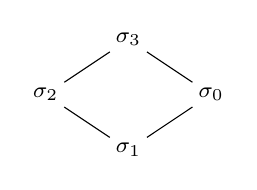
\begin{tikzpicture}[baseline=(current bounding box.center),every node/.style={font=\footnotesize, inner sep=2pt}]
\node (t) at (0,1.4) {$\sigma_3$};
\node (l) at (-1.05,0.7) {$\sigma_2$};
\node (r) at (1.05,0.7) {$\sigma_0$};
\node (b) at (0,0) {$\sigma_1$};
\draw (t)--(l); \draw (t)--(r); \draw (l)--(b); \draw (r)--(b);
\end{tikzpicture}
\]
这里各个 $\sigma_i$ 是 $\mathrm{PS}(\xi)$ 的 Jordan--Hölder 因子；图中各行是它的基座滤过（socle filtration）的层（从图的底部数起），等价地，是余基座滤过（cosocle filtration）的层（从图的顶部数起）；连线表示非平凡的扩张。

写 $\CC_i:=\CC_{\sigma_i}$；我们现在的目标是描述 $\CC_0\cup\CC_1\cup\CC_2\cup\CC_3$，然后描述其 Picard 群。我们首先注意，此并容许开覆盖
\ysrc{319}\begin{equation}\tag{7.7.20}\label{eq:a4-7-7-20}
\begin{aligned}
\{&D(u_0x_0),\;D(v_1y_1),\;D(u_2x_2),\;D(v_3y_3),\;D(v_0x_0)\cup D(u_1y_1),\\
&D(v_1x_1)\cup D(u_2y_2),\;D(v_2x_2)\cup D(u_3y_3),\;D(v_3x_3)\cup D(u_0y_0),\\
&D(v_0y_0)\cup D(u_1x_1)\cup D(v_2y_2)\cup D(u_3x_3)\}.
\end{aligned}
\end{equation}
（这里及下文沿用 $u,v,x,y,a,b$ 的记号，但加下标 $i\in\{0,1,2,3\}$ 以指明变量所属的成分。）以下是这些开子集的显式描述：
\[
D(u_ix_i)=(\GG_m)_{u_i/x_i}\times[\mathbf A^2_{v_i,y_i}/(\GG_m)_{b_i}],\qquad
D(v_iy_i)=[\mathbf A^2_{u_i,x_i}/(\GG_m)_{a_i}]\times(\GG_m)_{v_iy_i};
\]
\[
D(v_ix_i)=\mathbf A^1_{u_i/x_i}\times\mathbf A^1_{v_iy_i},\qquad
D(u_{i+1}y_{i+1})=\mathbf A^1_{x_{i+1}/u_{i+1}}\times\mathbf A^1_{v_{i+1}y_{i+1}},
\]
并且对 $i=0,2$，有
\[
D(v_ix_i)\cup D(u_{i+1}y_{i+1})=\{(u_i/x_i,v_iy_i,v_{i+1}y_{i+1})\mid (u_i/x_i)(v_{i+1}y_{i+1})=0\},
\]
连同等同 $v_iy_i=x_{i+1}/u_{i+1}$；而对 $i=1,3$，有
\[
D(v_ix_i)\cup D(u_{i+1}y_{i+1})=\{(u_i/x_i,v_iy_i,x_{i+1}/u_{i+1})\mid (v_iy_i)(x_{i+1}/u_{i+1})=0\},
\]
连同等同 $u_i/x_i=v_{i+1}y_{i+1}$；最后
\[
\begin{aligned}
& D(v_0y_0)\cup D(u_1x_1)\cup D(v_2y_2)\cup D(u_3x_3)\\
&=[\{(u_0,x_0,v_1,y_3,v_0y_0)\mid u_0v_1=x_0y_3=0,\ v_0y_0\neq0\}/(\GG_m)_{a_0}],
\end{aligned}
\]
其中我们有等同
\[
x_0=y_1,\quad x_2=y_3,\quad u_0=v_3,\quad u_2=v_1,
\]
\[
v_0y_0=x_1/u_1=(v_2y_2)^{-1}=u_3/x_3,\qquad a_0=b_1^{-1}=a_2^{-1}=b_3.
\]
利用开覆盖 (7.7.20)，我们计算
\begin{equation}\tag{7.7.21}\label{eq:a4-7-7-21}
\Gamma(\OO_{\CC_0\cup\CC_1\cup\CC_2\cup\CC_3})=k[v_1y_1,v_3y_3]/(v_1y_1v_3y_3).
\end{equation}
（稍作说明：函数 $v_1y_1$ 在 $\CC_1$ 上良定义，并零延拓到四个成分之并上。类似地，函数 $v_3y_3$ 在 $\CC_3$ 上良定义，也零延拓。）

可以证明存在嵌入
\begin{equation}\tag{7.7.22}\label{eq:a4-7-7-22}
\mathrm{Pic}(\CC_0\cup\CC_1\cup\CC_2\cup\CC_3)\hookrightarrow\Z\times\Z\times\Z\times\Z\times\Z,
\end{equation}
其中各因子分别由 $\mathrm{Pic}(D(v_1y_1))$、$\mathrm{Pic}(D(v_3y_3))$、$\mathrm{Pic}\bigl(D(v_0y_0)\cup D(u_1x_1)\cup D(v_2y_2)\cup D(u_3x_3)\bigr)$、$\mathrm{Pic}(D(u_0x_0))$ 与 $\mathrm{Pic}(D(u_2x_2))$ 给出，态射由限制定义。此嵌入的像等于
\begin{equation}\tag{7.7.23}\label{eq:a4-7-7-23}
\{(j,k,l,m,n)\mid j-k+m-n=0\};
\end{equation}
特别地，$\mathrm{Pic}(\CC_0\cup\CC_1\cup\CC_2\cup\CC_3)\cong\Z^4$。

要精确固定坐标的选取，最简单的办法是描述相应的嵌入
\begin{equation}\tag{7.7.24}\label{eq:a4-7-7-24}
\mathrm{Pic}(\CC_0\cup\CC_1\cup\CC_2\cup\CC_3)\hookrightarrow\mathrm{Pic}(\CC_0)\times\mathrm{Pic}(\CC_1)\times\mathrm{Pic}(\CC_2)\times\mathrm{Pic}(\CC_3);
\end{equation}
\ysrc{320}它由
\begin{equation}\tag{7.7.25}\label{eq:a4-7-7-25}
(j,k,l,m,n)\mapsto\bigl((l,m),(j,-l),(-l,n),(k,l)\bigr)
\end{equation}
给出。

\begin{exam}{7.7.26}\label{thm:a4-7-7-26}
我们有如下 $\OO_{\CC_0\cup\CC_1\cup\CC_2\cup\CC_3}$ 的理想子层图：
\begin{center}
\begin{tikzcd}[row sep=1.05cm, column sep=0.55cm, cells={font=\footnotesize}]
 & \OO_{\CC_0\cup\CC_1\cup\CC_2\cup\CC_3} & & & \\
 & \mathcal I_{\CC_3} \arrow[u, hook, "{\OO_{\CC_3}}"] \arrow[r, equal] & \mathcal I_{\CC_2\cup\CC_3}+\mathcal I_{\CC_0\cup\CC_3} & & \\
\mathcal I_{\CC_2\cup\CC_3} \arrow[ur, hook, "{\OO_{\CC_2}(-1,0)}" pos=0.42] & & \mathcal I_{\CC_0\cup\CC_3} \arrow[ul, hook, "{\OO_{\CC_0}(-1,0)}" pos=0.58] & & \\
 & \mathcal I_{\CC_0\cup\CC_2\cup\CC_3} \arrow[ul, hook] \arrow[ur, hook] \arrow[r, equal] & \mathcal I_{\CC_2\cup\CC_3}\cap\mathcal I_{\CC_0\cup\CC_3} \arrow[r, equal] & v_1y_1\OO_{\CC_0\cup\CC_1\cup\CC_2\cup\CC_3} & \OO_{\CC_1} \arrow[l, hook', "{\sim}" below, "{v_1y_1\cdot}" above]
\end{tikzcd}
\end{center}
其中箭头上的层标号表示相应的余核\tn{底本此句作「where the sheaf labels on the arrows are indicate the corresponding cokernel」，其中「are indicate」语法不谐；译文按原意处理。上下文推断，无外部依据。}。于是可以用如下扩张图描述 $\OO_{\CC_0\cup\CC_1\cup\CC_2\cup\CC_3}$：
\begin{equation}\tag{7.7.27}\label{eq:a4-7-7-27}
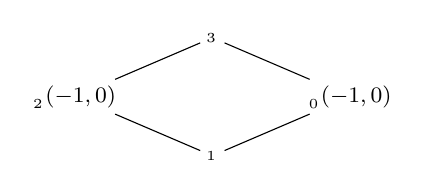
\begin{tikzpicture}[baseline=(current bounding box.center),every node/.style={font=\footnotesize, inner sep=2pt}]
\node (t) at (0,1.5) {$\OO_{\CC_3}$};
\node (l) at (-1.75,0.75) {$\OO_{\CC_2}(-1,0)$};
\node (r) at (1.75,0.75) {$\OO_{\CC_0}(-1,0)$};
\node (b) at (0,0) {$\OO_{\CC_1}$};
\draw (t)--(l); \draw (t)--(r); \draw (l)--(b); \draw (r)--(b);
\end{tikzpicture}
\end{equation}
类似地，我们有图
\begin{center}
\begin{tikzcd}[row sep=1.05cm, column sep=0.55cm, cells={font=\footnotesize}]
 & \OO_{\CC_0\cup\CC_1\cup\CC_2\cup\CC_3} & & & \\
 & \mathcal I_{\CC_1} \arrow[u, hook, "{\OO_{\CC_1}}"] \arrow[r, equal] & \mathcal I_{\CC_0\cup\CC_1}+\mathcal I_{\CC_1\cup\CC_2} & & \\
\mathcal I_{\CC_0\cup\CC_1} \arrow[ur, hook, "{\OO_{\CC_0}(-1,0)}" pos=0.42] & & \mathcal I_{\CC_1\cup\CC_2} \arrow[ul, hook, "{\OO_{\CC_2}(-1,0)}" pos=0.58] & & \\
 & \mathcal I_{\CC_0\cup\CC_1\cup\CC_2} \arrow[ul, hook] \arrow[ur, hook] \arrow[r, equal] & \mathcal I_{\CC_0\cup\CC_1}\cap\mathcal I_{\CC_1\cup\CC_2} \arrow[r, equal] & v_3y_3\OO_{\CC_0\cup\CC_1\cup\CC_2\cup\CC_3} & \OO_{\CC_3} \arrow[l, hook', "{\sim}" below, "{v_3y_3\cdot}" above]
\end{tikzcd}
\end{center}
\ysrc{321}由此可以用如下扩张图描述 $\OO_{\CC_0\cup\CC_1\cup\CC_2\cup\CC_3}$：
\begin{equation}\tag{7.7.28}\label{eq:a4-7-7-28}
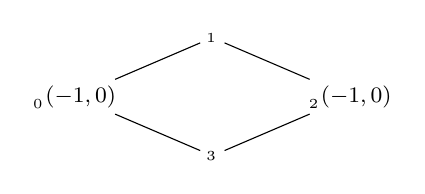
\begin{tikzpicture}[baseline=(current bounding box.center),every node/.style={font=\footnotesize, inner sep=2pt}]
\node (t) at (0,1.5) {$\OO_{\CC_1}$};
\node (l) at (-1.75,0.75) {$\OO_{\CC_0}(-1,0)$};
\node (r) at (1.75,0.75) {$\OO_{\CC_2}(-1,0)$};
\node (b) at (0,0) {$\OO_{\CC_3}$};
\draw (t)--(l); \draw (t)--(r); \draw (l)--(b); \draw (r)--(b);
\end{tikzpicture}
\end{equation}
\end{exam}

\begin{exam}{7.7.29}\label{thm:a4-7-7-29}
我们还有如下 $\OO_{\CC_0\cup\CC_1\cup\CC_2\cup\CC_3}$ 的理想子层图，即
\begin{center}
\begin{tikzcd}[row sep=1.05cm, column sep=0.55cm, cells={font=\footnotesize}]
 & \OO_{\CC_0\cup\CC_1\cup\CC_2\cup\CC_3} & & & \\
 & \mathcal I_{\CC_0} \arrow[u, hook, "{\OO_{\CC_0}}"] \arrow[r, equal] & \mathcal I_{\CC_0\cup\CC_3}+\mathcal I_{\CC_0\cup\CC_1} & & \\
\mathcal I_{\CC_0\cup\CC_3} \arrow[ur, hook, "{\OO_{\CC_3}(0,1)}" pos=0.42] & & \mathcal I_{\CC_0\cup\CC_1} \arrow[ul, hook, "{\OO_{\CC_1}(0,-1)}" pos=0.58] & & \\
 & \mathcal I_{\CC_0\cup\CC_1\cup\CC_3} \arrow[ul, hook] \arrow[ur, hook] \arrow[r, equal] & \mathcal I_{\CC_0\cup\CC_3}\cap\mathcal I_{\CC_0\cup\CC_1} & \OO_{\CC_2}(-2,0) \arrow[l, hook', "{\sim}" below] & 
\end{tikzcd}
\end{center}
与
\begin{center}
\begin{tikzcd}[row sep=1.05cm, column sep=0.55cm, cells={font=\footnotesize}]
 & \OO_{\CC_0\cup\CC_1\cup\CC_2\cup\CC_3} & & & \\
 & \mathcal I_{\CC_2} \arrow[u, hook, "{\OO_{\CC_2}}"] \arrow[r, equal] & \mathcal I_{\CC_1\cup\CC_2}+\mathcal I_{\CC_2\cup\CC_3} & & \\
\mathcal I_{\CC_1\cup\CC_2} \arrow[ur, hook, "{\OO_{\CC_1}(0,1)}" pos=0.42] & & \mathcal I_{\CC_2\cup\CC_3} \arrow[ul, hook, "{\OO_{\CC_3}(0,-1)}" pos=0.58] & & \\
 & \mathcal I_{\CC_1\cup\CC_2\cup\CC_3} \arrow[ul, hook] \arrow[ur, hook] \arrow[r, equal] & \mathcal I_{\CC_1\cup\CC_2}\cap\mathcal I_{\CC_2\cup\CC_3} & \OO_{\CC_0}(-2,0) \arrow[l, hook', "{\sim}" below] & 
\end{tikzcd}
\end{center}
由此可以用如下扩张图描述 $\OO_{\CC_0\cup\CC_1\cup\CC_2\cup\CC_3}$：
\begin{equation}\tag{7.7.30}\label{eq:a4-7-7-30}
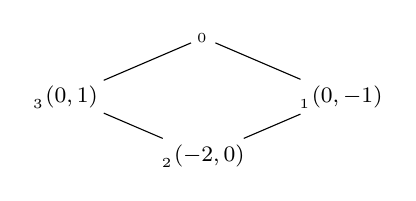
\begin{tikzpicture}[baseline=(current bounding box.center),every node/.style={font=\footnotesize, inner sep=2pt}]
\node (t) at (0,1.5) {$\OO_{\CC_0}$};
\node (l) at (-1.75,0.75) {$\OO_{\CC_3}(0,1)$};
\node (r) at (1.75,0.75) {$\OO_{\CC_1}(0,-1)$};
\node (b) at (0,0) {$\OO_{\CC_2}(-2,0)$};
\draw (t)--(l); \draw (t)--(r); \draw (l)--(b); \draw (r)--(b);
\end{tikzpicture}
\end{equation}
\ysrc{322}与
\begin{equation}\tag{7.7.31}\label{eq:a4-7-7-31}
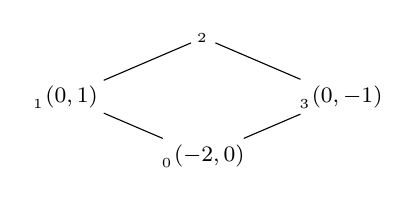
\begin{tikzpicture}[baseline=(current bounding box.center),every node/.style={font=\footnotesize, inner sep=2pt}]
\node (t) at (0,1.5) {$\OO_{\CC_2}$};
\node (l) at (-1.75,0.75) {$\OO_{\CC_1}(0,1)$};
\node (r) at (1.75,0.75) {$\OO_{\CC_3}(0,-1)$};
\node (b) at (0,0) {$\OO_{\CC_0}(-2,0)$};
\draw (t)--(l); \draw (t)--(r); \draw (l)--(b); \draw (r)--(b);
\end{tikzpicture}
\end{equation}
\end{exam}

现在我们解释上述计算的表示论含义。我们写 $U:=\mathrm{PS}(\xi)$，并回忆用其 Jordan--Hölder 因子对 $U$ 的描述
\begin{equation}\tag{7.7.32}\label{eq:a4-7-7-32}
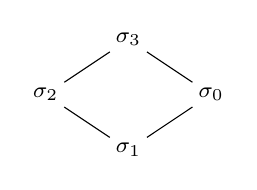
\begin{tikzpicture}[baseline=(current bounding box.center),every node/.style={font=\footnotesize, inner sep=2pt}]
\node (t) at (0,1.4) {$\sigma_3$};
\node (l) at (-1.05,0.7) {$\sigma_2$};
\node (r) at (1.05,0.7) {$\sigma_0$};
\node (b) at (0,0) {$\sigma_1$};
\draw (t)--(l); \draw (t)--(r); \draw (l)--(b); \draw (r)--(b);
\end{tikzpicture}
\end{equation}
于是定义
\[
\mathfrak A(c\text{-}\mathrm{Ind}^G_{KZ}U):=\OO_{\CC_0\cup\CC_1\cup\CC_2\cup\CC_3}(-1,-1,0,0,0),
\]
其中扭按嵌入 (7.7.22) 来理解；注意 $-1-(-1)+0=0=0$\tn{底本此处作 $-1-(-1)+0=0=0$；按 (7.7.23) 的约束 $j-k+m-n=0$，此式应为 $-1-(-1)+0-0=0$，疑排版时漏掉 $-0$；译文照录原文。上下文推断，无外部依据。}，因此 (7.7.23) 的约束得到满足。若对图 (7.7.27) 作相应的扭，并计入 (7.7.25) 的公式，则得到图
\begin{equation}\tag{7.7.33}\label{eq:a4-7-7-33}
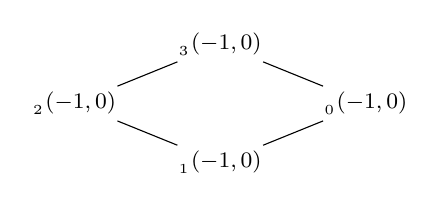
\begin{tikzpicture}[baseline=(current bounding box.center),every node/.style={font=\footnotesize, inner sep=2pt}]
\node (t) at (0,1.5) {$\OO_{\CC_3}(-1,0)$};
\node (l) at (-1.85,0.75) {$\OO_{\CC_2}(-1,0)$};
\node (r) at (1.85,0.75) {$\OO_{\CC_0}(-1,0)$};
\node (b) at (0,0) {$\OO_{\CC_1}(-1,0)$};
\draw (t)--(l); \draw (t)--(r); \draw (l)--(b); \draw (r)--(b);
\end{tikzpicture}
\end{equation}
它表明我们的定义与 $\mathfrak A$ 的函子性以及图 (7.7.32) 相容。

若改为诱导特征 $\xi^s$（$\xi$ 的非平凡 Weyl 群共轭），则得到表示 $U^s:=\mathrm{PS}(\xi^s)$，它可由如下扩张图描述：
\begin{equation}\tag{7.7.34}\label{eq:a4-7-7-34}
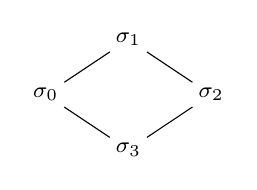
\begin{tikzpicture}[baseline=(current bounding box.center),every node/.style={font=\footnotesize, inner sep=2pt}]
\node (t) at (0,1.4) {$\sigma_1$};
\node (l) at (-1.05,0.7) {$\sigma_0$};
\node (r) at (1.05,0.7) {$\sigma_2$};
\node (b) at (0,0) {$\sigma_3$};
\draw (t)--(l); \draw (t)--(r); \draw (l)--(b); \draw (r)--(b);
\end{tikzpicture}
\end{equation}

% 本片止于印刷页 322 页末（§7.7.19）。续片自 PDF 336 页（印刷页 323）起。
